\documentclass[3p,times,10pt,authoryear]{elsarticle}
\usepackage[T1]{fontenc}
\usepackage[utf8]{inputenc}
\usepackage{amsmath,amssymb}
\usepackage{graphicx,booktabs,multirow,array,tabularx,makecell}
\usepackage[table,dvipsnames]{xcolor}
\usepackage{enumitem,microtype,textcomp}
\providecommand{\euro}{\texteuro}
\usepackage{placeins}
\usepackage[labelfont=bf,labelsep=period,font=small,skip=4pt]{caption}
\usepackage[colorlinks=true,linkcolor=MidnightBlue,citecolor=MidnightBlue,urlcolor=MidnightBlue]{hyperref}
\usepackage[capitalise,nameinlink]{cleveref}
\graphicspath{{fig/}}
% auto-generated by pipeline/paper_numbers.py -- do not edit
\newcommand{\nFT}{1\,075\,585}
\newcommand{\nTech}{25\,755}
\newcommand{\nAI}{8\,131}
\newcommand{\nCore}{1\,096}
\newcommand{\nCSP}{1\,614\,346}
\newcommand{\nHN}{91\,851}
\newcommand{\nAll}{2.8}
\newcommand{\pTech}{2.39}
\newcommand{\pAI}{0.76}
\newcommand{\pCore}{0.10}
\newcommand{\nAIoutside}{4\,490}
\newcommand{\pAIoutside}{55}
\newcommand{\salCore}{47.5}
\newcommand{\salNCore}{242}
\newcommand{\expCore}{47}
\newcommand{\cdiCore}{53}
\newcommand{\idfCore}{39}
\newcommand{\nSegCore}{1\,096}
\newcommand{\salAItech}{50.0}
\newcommand{\salNAItech}{536}
\newcommand{\expAItech}{71}
\newcommand{\cdiAItech}{64}
\newcommand{\idfAItech}{29}
\newcommand{\nSegAItech}{2\,545}
\newcommand{\salTech}{39.0}
\newcommand{\salNTech}{7\,235}
\newcommand{\expTech}{60}
\newcommand{\cdiTech}{69}
\newcommand{\idfTech}{25}
\newcommand{\nSegTech}{22\,305}
\newcommand{\salAIother}{35.0}
\newcommand{\salNAIother}{1\,253}
\newcommand{\expAIother}{63}
\newcommand{\cdiAIother}{54}
\newcommand{\idfAIother}{23}
\newcommand{\nSegAIother}{4\,490}
\newcommand{\salRest}{24.4}
\newcommand{\salNRest}{467\,759}
\newcommand{\expRest}{48}
\newcommand{\cdiRest}{51}
\newcommand{\idfRest}{11}
\newcommand{\nSegRest}{1\,045\,149}
\newcommand{\salAll}{24.4}
\newcommand{\salPremAItech}{28}
\newcommand{\hnAIlast}{58}
\newcommand{\hnAIpre}{18}
\newcommand{\hnCorelast}{13}
\newcommand{\hnCorepre}{4}
\newcommand{\hnAIfirst}{4}
\newcommand{\hnLastMonth}{2026-10}
\newcommand{\hnTitlesPre}{7.0}
\newcommand{\hnTitlesLast}{16.8}
\newcommand{\cspFirst}{9.6}
\newcommand{\cspLast}{24.3}
\newcommand{\cspRatio}{2.5}
\newcommand{\cspAIn}{2\,973}
\newcommand{\nafJ}{5.2}
\newcommand{\nafL}{2.3}
\newcommand{\nafM}{1.7}
\newcommand{\nafF}{0.14}
\newcommand{\idfShare}{1.7}
\newcommand{\idfConc}{31}
\newcommand{\idfJobs}{12}
\newcommand{\regSecond}{Occitanie}
\newcommand{\regSecondShare}{0.7}
\newcommand{\conLIB}{8.3}
\newcommand{\conCDI}{0.84}
\newcommand{\conMIS}{0.13}
\newcommand{\conCDD}{0.68}
\newcommand{\depHautsDeSeine}{3.66}
\newcommand{\depParis}{2.87}
\newcommand{\topTenEmp}{12.4}
\newcommand{\topEmp}{Collective.work}
\newcommand{\topEmpN}{508}
\newcommand{\EForwardDeployedEngineer}{0.80}
\newcommand{\stageForwardDeployedEngineer}{diffusing}
\newcommand{\firstForwardDeployedEngineer}{2018-08}
\newcommand{\hnLastForwardDeployedEngineer}{33}
\newcommand{\hnPrevForwardDeployedEngineer}{17}
\newcommand{\frForwardDeployedEngineer}{9}
\newcommand{\frEmpForwardDeployedEngineer}{2}
\newcommand{\gForwardDeployedEngineer}{+0.64}
\newcommand{\EAiEngineer}{0.82}
\newcommand{\stageAiEngineer}{established}
\newcommand{\firstAiEngineer}{2017-03}
\newcommand{\hnLastAiEngineer}{125}
\newcommand{\hnPrevAiEngineer}{121}
\newcommand{\frAiEngineer}{229}
\newcommand{\frEmpAiEngineer}{70}
\newcommand{\gAiEngineer}{+0.03}
\newcommand{\EAgentEngineer}{0.43}
\newcommand{\stageAgentEngineer}{appearing}
\newcommand{\firstAgentEngineer}{2025-08}
\newcommand{\hnLastAgentEngineer}{3}
\newcommand{\hnPrevAgentEngineer}{6}
\newcommand{\frAgentEngineer}{40}
\newcommand{\frEmpAgentEngineer}{10}
\newcommand{\gAgentEngineer}{-0.56}
\newcommand{\EGenaiEngineer}{0.49}
\newcommand{\stageGenaiEngineer}{fading}
\newcommand{\firstGenaiEngineer}{2023-10}
\newcommand{\hnLastGenaiEngineer}{4}
\newcommand{\hnPrevGenaiEngineer}{12}
\newcommand{\frGenaiEngineer}{33}
\newcommand{\frEmpGenaiEngineer}{15}
\newcommand{\gGenaiEngineer}{-0.96}
\newcommand{\EAiArchitect}{0.65}
\newcommand{\stageAiArchitect}{appearing}
\newcommand{\firstAiArchitect}{2026-03}
\newcommand{\hnLastAiArchitect}{4}
\newcommand{\hnPrevAiArchitect}{0}
\newcommand{\frAiArchitect}{45}
\newcommand{\frEmpAiArchitect}{13}
\newcommand{\gAiArchitect}{+1.61}
\newcommand{\EAiGovernance}{0.44}
\newcommand{\stageAiGovernance}{appearing}
\newcommand{\firstAiGovernance}{2025-02}
\newcommand{\hnLastAiGovernance}{5}
\newcommand{\hnPrevAiGovernance}{7}
\newcommand{\frAiGovernance}{10}
\newcommand{\frEmpAiGovernance}{4}
\newcommand{\gAiGovernance}{-0.29}
\newcommand{\EMlEngineer}{0.54}
\newcommand{\stageMlEngineer}{established}
\newcommand{\firstMlEngineer}{2015-09}
\newcommand{\hnLastMlEngineer}{68}
\newcommand{\hnPrevMlEngineer}{97}
\newcommand{\frMlEngineer}{28}
\newcommand{\frEmpMlEngineer}{9}
\newcommand{\gMlEngineer}{-0.35}
\newcommand{\EDataScientist}{0.51}
\newcommand{\stageDataScientist}{established}
\newcommand{\firstDataScientist}{2013-03}
\newcommand{\hnLastDataScientist}{21}
\newcommand{\hnPrevDataScientist}{23}
\newcommand{\frDataScientist}{139}
\newcommand{\frEmpDataScientist}{41}
\newcommand{\gDataScientist}{-0.09}
\newcommand{\EDataEngineer}{0.51}
\newcommand{\stageDataEngineer}{established}
\newcommand{\firstDataEngineer}{2013-04}
\newcommand{\hnLastDataEngineer}{47}
\newcommand{\hnPrevDataEngineer}{54}
\newcommand{\frDataEngineer}{413}
\newcommand{\frEmpDataEngineer}{94}
\newcommand{\gDataEngineer}{-0.14}
\newcommand{\EPromptEngineer}{0.38}
\newcommand{\stagePromptEngineer}{too rare}
\newcommand{\firstPromptEngineer}{--}
\newcommand{\hnLastPromptEngineer}{0}
\newcommand{\hnPrevPromptEngineer}{0}
\newcommand{\frPromptEngineer}{1}
\newcommand{\frEmpPromptEngineer}{0}
\newcommand{\gPromptEngineer}{+0.00}
\newcommand{\EMlopsEngineer}{0.58}
\newcommand{\stageMlopsEngineer}{diffusing}
\newcommand{\firstMlopsEngineer}{2021-09}
\newcommand{\hnLastMlopsEngineer}{7}
\newcommand{\hnPrevMlopsEngineer}{6}
\newcommand{\frMlopsEngineer}{30}
\newcommand{\frEmpMlopsEngineer}{8}
\newcommand{\gMlopsEngineer}{+0.13}
\newcommand{\EHeadOfAi}{0.70}
\newcommand{\stageHeadOfAi}{diffusing}
\newcommand{\firstHeadOfAi}{2018-02}
\newcommand{\hnLastHeadOfAi}{20}
\newcommand{\hnPrevHeadOfAi}{16}
\newcommand{\frHeadOfAi}{112}
\newcommand{\frEmpHeadOfAi}{36}
\newcommand{\gHeadOfAi}{+0.21}
\newcommand{\nStages}{22}
\newcommand{\nAppearing}{3}
\newcommand{\nFading}{1}
\newcommand{\nEstablished}{5}
\newcommand{\nDiffusing}{6}
\newcommand{\nNgramsHN}{392}
\newcommand{\nNgramsNew}{28}
\newcommand{\nCanonFR}{2\,393}
\newcommand{\nCanonTitles}{23}
\newcommand{\skModelCore}{41}
\newcommand{\skGenAICore}{61}
\newcommand{\skCloudCore}{56}
\newcommand{\skSoftCore}{61}
\newcommand{\skGovCore}{21}
\newcommand{\skDataEngCore}{32}
\newcommand{\skTransvCore}{54}
\newcommand{\skModelAItech}{22}
\newcommand{\skGenAIAItech}{35}
\newcommand{\skCloudAItech}{63}
\newcommand{\skSoftAItech}{74}
\newcommand{\skGovAItech}{15}
\newcommand{\skDataEngAItech}{35}
\newcommand{\skTransvAItech}{54}
\newcommand{\skModelTech}{7}
\newcommand{\skGenAITech}{0}
\newcommand{\skCloudTech}{42}
\newcommand{\skSoftTech}{44}
\newcommand{\skGovTech}{11}
\newcommand{\skDataEngTech}{17}
\newcommand{\skTransvTech}{51}
\newcommand{\hnGenAIpre}{5}
\newcommand{\hnGenAIlast}{39}
\newcommand{\hnModelPre}{76}
\newcommand{\hnModelLast}{20}
\newcommand{\hnGovLast}{5}
\newcommand{\precIsTech}{88}
\newcommand{\recIsTech}{92}
\newcommand{\fIsTech}{0.90}
\newcommand{\kappaIsTech}{0.78}
\newcommand{\nValIsTech}{1\,000}
\newcommand{\precAiAny}{90}
\newcommand{\recAiAny}{98}
\newcommand{\fAiAny}{0.94}
\newcommand{\kappaAiAny}{0.86}
\newcommand{\nValAiAny}{1\,000}
\newcommand{\precAiCore}{79}
\newcommand{\recAiCore}{96}
\newcommand{\fAiCore}{0.86}
\newcommand{\kappaAiCore}{0.81}
\newcommand{\nValAiCore}{1\,000}
\newcommand{\precAItext}{84}
\newcommand{\canonAgree}{67}
\newcommand{\nCanonBoth}{287}
\newcommand{\nJudged}{1000}
\newcommand{\aiJobShare}{87}

\setlist{itemsep=1pt,topsep=2pt,parsep=0pt,leftmargin=1.6em}
\setlength{\textfloatsep}{9pt plus 2pt minus 2pt}
\setlength{\floatsep}{8pt plus 2pt minus 2pt}
\setlength{\intextsep}{8pt plus 2pt minus 2pt}
\renewcommand{\arraystretch}{1.08}
\setlength{\tabcolsep}{4.2pt}
\definecolor{tgt}{HTML}{2255CC}
\newcommand{\tg}[1]{\textcolor{tgt}{#1\textsuperscript{\dag}}}
\newcommand{\RQ}[1]{\textbf{RQ#1}}
\journal{Technological Forecasting and Social Change}

\begin{document}
\begin{frontmatter}
\title{Where do new AI jobs come from? Measuring the emergence, diffusion and lifecycle of artificial-intelligence occupations from \nAll{} million job postings in France and fifteen years of international tech hiring}

\author[elia,eiffel]{Linda Belkessa\corref{cor1}}
\ead{linda.belkessa@univ-eiffel.fr}
\author[elia]{Armand Derhy}
\author[eiffel,elia]{Mahdi Zargayouna}
\cortext[cor1]{Corresponding author.}
\affiliation[elia]{organization={Laboratoire ELIA, Paris School of Technology \& Business},city={Paris},postcode={75011},country={France}}
\affiliation[eiffel]{organization={COSYS-GRETTIA, Universit\'e Gustave Eiffel},city={Marne-la-Vall\'ee},postcode={77447},country={France}}

\begin{abstract}
New occupations are usually identified years after they appear, when statistical classifications catch up with the labour market. Online job postings make it possible to observe the birth, spread and decline of a job title month by month. This study builds an open corpus of \nAll{} million job postings, \nFT{} offers published through the French public employment service in 2026 with their full text, \nCSP{} public-sector postings from 2022 to 2026 and \nHN{} international technology hiring posts from 2011 to 2026, and applies rules fixed before any result was read to isolate technology jobs, jobs that mention artificial intelligence (AI) and jobs whose title is an AI title. We propose an Emergence Index that combines, for each canonical title, its novelty, twelve-month growth, breadth across employers and territories, and persistence, and we assign each title to a lifecycle stage. Internationally, the share of tech hiring posts that mention AI rose from \hnAIpre\,\% in the twelve months before ChatGPT to \hnAIlast\,\% in the last twelve months, and the share of posts whose role title is an AI title from \hnCorepre\,\% to \hnCorelast\,\%. In France, AI is mentioned in \pAI\,\% of all postings and \pCore\,\% carry an AI title; \pAIoutside\,\% of the postings that mention AI are not technology jobs, and the share is highest in freelance missions (\conLIB\,\%), in information and communication (\nafJ\,\%) and in \^Ile-de-France (\idfShare\,\%). Postings that combine a technology job with AI advertise a median salary of \salAItech\,k\euro{} against \salTech\,k\euro{} for other technology jobs, a premium of \salPremAItech\,\%. Most titles that appeared after 2022 are relabellings of machine-learning roles; a minority (forward deployed engineer, AI agent engineer, AI governance) combine new skill profiles with fast diffusion across employers, while prompt engineering has already faded. In the French public sector, AI mentions per 10\,000 postings grew \cspRatio-fold between 2022 and 2026. A blind annotation of 1\,000 postings by a language-model judge gives a precision of \precAiAny\,\% and a recall of \recAiAny\,\% for the AI-mention rule. The corpus, the lexicon and the index are released with a monthly observatory.
\end{abstract}

\begin{keyword}
Emerging occupations \sep Artificial intelligence \sep Online job advertisements \sep Skills \sep Labour demand \sep France
\end{keyword}
\end{frontmatter}

\noindent\fcolorbox{tgt}{white}{\parbox{\dimexpr\textwidth-2\fboxsep-2\fboxrule}{\footnotesize\textbf{Status of this draft (14 October 2026).} All numbers are measured on the corpus frozen on 14 October 2026 and regenerated automatically from the result tables. The French series covers 2026 only; the daily harvest that started on 14 October 2026 and the archival reconstruction described in \cref{sec:data} will extend it before submission. Numbers in \textcolor{tgt}{blue with a dagger (\dag)} are targets for analyses not yet run.}}

\section{Introduction}\label{sec:intro}
Most of what we know about new work comes from censuses and occupational classifications, which record a new occupation once it is large enough to be coded. \citet{lin2011} and \citet{autor2024} show that more than half of today's jobs did not exist in 1940 and that new work arises where new technologies meet existing skills. This evidence is precise about decades and silent about months. The current wave of artificial intelligence (AI) is different in one respect: employers describe the jobs they create in online postings, in their own words, within days. The job titles of 2024 and 2025, forward deployed engineer, AI agent engineer, generative AI engineer or AI governance officer, appeared in postings long before any classification registered them. French statistics are a case in point: the ROME~4.0 repository added a fiche for AI engineers in 2026 \citep{rome2026}, and no official source yet counts the titles that employers use.

Online job advertisements (OJA) have become the standard instrument for measuring AI labour demand. \citet{alekseeva2021} and \citet{acemoglu2022} document the rise of AI skills in United States vacancies, \citet{squicciarini2021} and \citet{borgonovi2023} extend the measurement to fourteen OECD countries, and \citet{bone2025} use eleven million United Kingdom vacancies to show that AI roles rely on skills more than on degrees. These studies measure the demand for AI \emph{skills}. They do not measure when a \emph{title} is born, how fast it spreads across employers and territories, when it stabilises and when it disappears, which is the object of the literature on new work. For France, the evidence rests on commercial aggregates \citep{pwc2025} or on European dashboards \citep{cedefop2019}, and no open corpus with full text exists.

In this study, we address this gap with an open, reproducible measurement of the emergence of AI occupations in France, placed against fifteen years of international technology hiring. More precisely, we answer five research questions:
\begin{itemize}[leftmargin=2.6em]
\item[\RQ{1}] Which AI job titles emerged since 2022, when did each appear, and are they new roles or relabelled ones?
\item[\RQ{2}] How fast do AI titles diffuse across employers, sectors, contract types and territories in France, and where is AI demanded outside technology jobs?
\item[\RQ{3}] What is the skill architecture of AI jobs, by family, and how does it differ from other technology jobs?
\item[\RQ{4}] Do AI jobs pay a premium and demand more experience than comparable technology jobs?
\item[\RQ{5}] Which titles are fading, and what does the French public sector show about diffusion beyond the private market?
\end{itemize}

Our approach proposes the following contributions:
\begin{enumerate}
\item We assemble a corpus of \nAll{} million postings from four open sources, with the full text of \nFT{} French offers, and we release the lexicon, the scope rules and the aggregated results. The rules were frozen before any result was read, and a blind annotation of 1\,000 postings by a language-model judge measures their precision and recall.
\item We define an \emph{Emergence Index} for job titles that combines novelty, twelve-month growth with shrinkage for small counts, breadth across employers and departments, and persistence, and we derive lifecycle stages (appearing, diffusing, established, fading) with explicit transition rules. The index is computed for \nStages{} canonical AI and data titles and complemented by a data-driven discovery of title n-grams.
\item We provide the first open cross-section of AI demand in France at the level of the posting, with sector, region, department, contract type, establishment size, salary and experience requirement, and the first public-sector series since 2022.
\item We show that the AI wave is visible in two layers that move at different speeds: a thin layer of AI-titled jobs and a thick layer of ordinary jobs that now mention AI, and that the second layer is largest outside technology occupations and in freelance missions.
\end{enumerate}

The remainder of the paper is organised as follows. \Cref{sec:lit} reviews the related work. \Cref{sec:data} describes the sources and the corpus. \Cref{sec:method} presents the scope rules, the canonical titles, the skill families and the Emergence Index. \Cref{sec:results} reports the results, \cref{sec:discussion} discusses their implications and limits, and \cref{sec:concl} concludes.

\section{Related work}\label{sec:lit}
\paragraph{New work and the birth of occupations} \citet{lin2011} measures new work through the titles added to the Dictionary of Occupational Titles and finds that it concentrates in cities with educated workers and a diverse industry mix. \citet{autor2024} extend the measurement to 1940--2018 and show that new work follows demand shocks and augmentation technologies, and that its content shifted from production to services. Both rely on official title lists updated every few years. Job postings bring the same question to a monthly resolution, at the cost of a noisier vocabulary.

\paragraph{AI exposure and AI demand} A first strand measures which occupations AI can affect \citep{frey2017,felten2021,eloundou2024,gmyrek2023}. A second strand measures what employers actually ask for. \citet{alekseeva2021} find that AI skills grew sharply across United States industries between 2010 and 2019 and carry a wage premium; \citet{acemoglu2022} show that AI-exposed establishments hire into AI positions and reduce other hiring; \citet{deming2018} relate posting requirements to firm wages. \citet{squicciarini2021} and \citet{borgonovi2023} report that AI-related postings remained below one per cent of all postings in most OECD countries in 2019--2022, which matches our French share. \citet{stephany2024} show that the value of a skill is set by its complementarity with other skills, with AI skills among the most valuable, and \citet{bone2025} find that university requirements for AI roles fell while AI skills command a premium. \citet{brynjolfsson2025} measure the productivity effect of generative AI at work. None of these studies tracks the lifecycle of a title.

\paragraph{Text mining of titles and skills} \citet{back2021} classify 480\,000 Finnish advertisements with an AI glossary; \citet{chiarello2021} compare ESCO with Industry~4.0 skills extracted from text; \citet{kim2026sao} forecast emerging jobs from subject--action--object triplets. Statistical offices have examined the representativeness of OJA against vacancy surveys \citep{beresewicz2021,cedefop2019}. Our contribution is to combine a title-level emergence measure with a skill-level description, on an open French corpus, and to validate the classification against blind annotations.

\section{Data}\label{sec:data}
\Cref{tab:corpus} describes the four sources. The France Travail API gives every offer published by the French public employment service with 36 fields, including the full description, the ROME~4.0 occupation code, the NAF sector, the contract type, the experience requirement, the posted salary range and the commune. We merged the live stock harvested on 14 October 2026 (476\,868 offers) with two archived dumps covering January to June 2026, removed duplicates by identifier, and obtained \nFT{} unique offers; 13\,\% of them share an identical text with another offer, which we keep because they are distinct vacancies. The public portal \emph{Choisir le Service Public} publishes every state, hospital and local-government vacancy since December 2022 with its title, occupation family and location, but without a description; we use \nCSP{} unique postings. The monthly \emph{Who is hiring} threads of Hacker News give \nHN{} international technology posts from April 2011 to October 2026, written by employers in a stable ``company $|$ role $|$ location'' format; this archive is our only source with a fifteen-year series. Adzuna's French IT category (11\,895 live ads) is used to check employer and salary patterns. Daily harvesting of the France Travail flow (about 20\,000 new offers per day) started on 14 October 2026, and an access request for the DARES JOCAS database of scraped French boards has been filed; both will extend the French series.

\begin{table}[t]
\centering\footnotesize
\caption{Corpus statement. Counts after deduplication by identifier. The France Travail corpus is a stock of live offers and two archived dumps, so its creation dates concentrate in April--October 2026. $^{a}$Posts truncated at 1\,100 characters by the crawler; titles and the first lines are complete.}\label{tab:corpus}
\begin{tabularx}{\textwidth}{@{}lllrlX@{}}
\toprule
Source & Coverage & Period & Postings & Text & Role in the study\\
\midrule
France Travail API v2 & France, all sectors & Jan--Oct 2026 & \nFT{} & full & cross-section: scope, skills, salaries, geography\\
Choisir le Service Public & French public sector & 2022--2026 & \nCSP{} & title & public-sector series\\
Hacker News ``Who is hiring'' & international tech & 2011--2026 & \nHN{} & full$^{a}$ & fifteen-year series, first appearance\\
Adzuna (IT category) & France, private boards & live, Oct 2026 & 11\,895 & 500 chars & validation of employers and salaries\\
\bottomrule
\end{tabularx}
\end{table}

Three limits of the sources matter for the interpretation. France Travail under-represents executive and technology jobs, which are advertised on specialised boards: technology occupations are \pTech\,\% of its offers. Its stock is censored by expiry, so creation dates cannot be used as a French time series yet. Hacker News is international, mostly North American, and written in English; it dates the birth of titles at the technological frontier rather than in France. No personal data is kept: contact fields are dropped at ingestion and employer names are used only for aggregate counts.

\section{Method}\label{sec:method}
\Cref{fig:pipeline} summarises the pipeline. Every rule below was written and frozen before the first result table was produced; the only later change corrected two sources of false positives found by the validation (the French verb form \emph{j'ai} matched by a case-insensitive ``AI'', and non-technology jobs filed under IT occupation codes), and the validation was rerun.

\begin{figure}[t]
\centering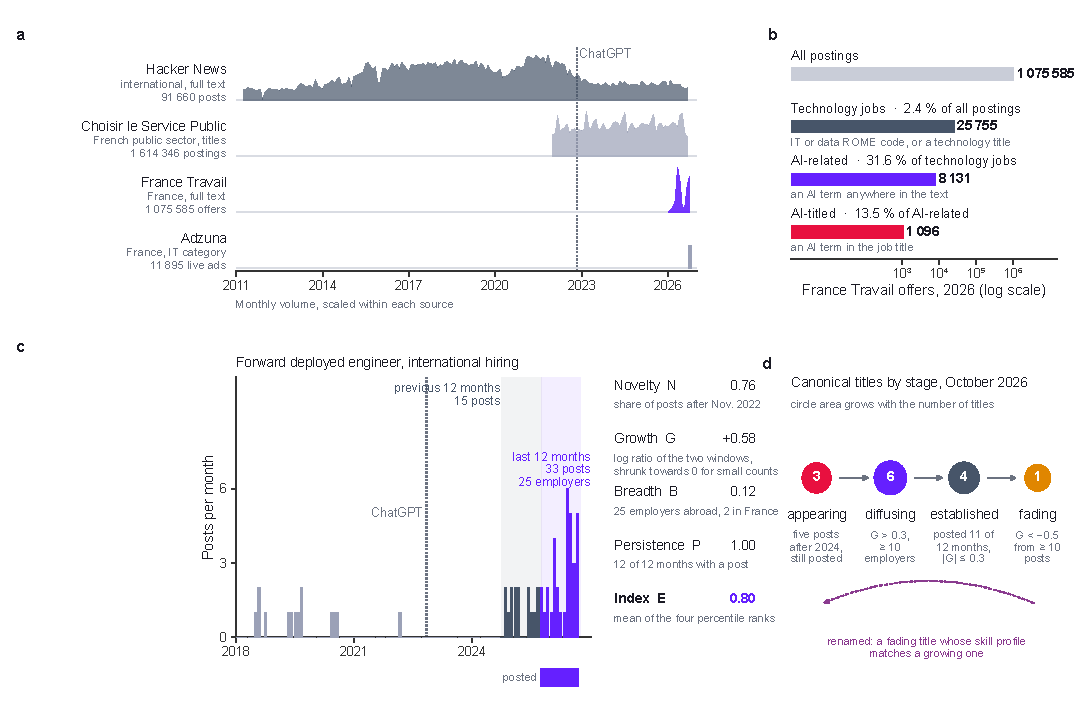
\includegraphics[width=\textwidth]{fig1_pipeline}
\caption{From four sources to the Emergence Index. The sources are merged once (A), labelled with scope rules frozen before any result was read (B), turned into monthly title series and the Emergence Index (C), and validated against blind annotations and external series (D).}\label{fig:pipeline}
\end{figure}

\subsection{Scope rules}\label{sec:scope}
Three nested sets are defined on each posting. \emph{Technology jobs} are postings whose ROME code belongs to the information-technology family (M18) or to the data occupations (M1405, M1419, M1423, M1435), or whose title matches a bilingual lexicon of technology roles (developer, software, DevOps, data engineer, cybersecurity, cloud, and so on), minus titles that are obviously not technology jobs although France Travail filed them under an IT code (business developer, restaurant \emph{serveur}, telecom field technician). \emph{AI-related} postings contain at least one term of a bilingual AI lexicon of 70 expressions (artificial intelligence, machine learning, deep learning, generative AI, LLM, NLP, computer vision, MLOps, RAG, prompt engineering, AI agents, and the main frameworks and model names), with explicit exclusions for homonyms; the acronyms IA and AI are matched in upper case only, which removes the French verb form and agency names such as ``IA Recrutement''. \emph{AI-core} postings carry an AI term in the title. For sensitivity analysis, a \emph{substantive} AI flag requires either an AI title, two distinct AI terms, or one technical term other than the bare acronym, a chatbot or a copilot.

\subsection{Canonical titles and skill families}\label{sec:titles}
Titles are normalised (gender marks, seniority tokens, locations and contract tokens removed, accents stripped) and mapped to 23 canonical AI and data titles by ordered regular expressions, from the most specific (forward deployed engineer, AI agent engineer, prompt engineer, generative AI engineer, MLOps engineer, NLP and computer-vision engineer) to the most generic (AI engineer, data scientist, data engineer, data analyst), grouped into eleven families. Titles that are AI-labelled but fit no canonical title are kept as ``other AI-labelled''. A data-driven discovery complements the list: every title bigram to 4-gram containing an AI token is counted with its first month, its last-twelve-month count and its employer breadth, and maximal n-grams are reported.

Skills are extracted with a dictionary of about 600 technologies and skills grouped into ten families (AI/ML modelling; generative AI and LLM; data engineering; software engineering; cloud, DevOps and MLOps; data analysis and BI; governance, ethics and regulation; product and project; domain; transversal and languages), matched with word boundaries in both languages; a list of over-generic words (\emph{environnement}, \emph{sécurité}, \emph{recherche}) is excluded because they match boilerplate. A second, embedding-based extractor against ESCO~1.2 \citep{esco2024} is planned for the revised version and is not used in the numbers below.

\subsection{Emergence Index and lifecycle stages}\label{sec:index}
For a canonical title $t$ observed monthly, let $n_{t,[a,b]}$ be its number of posts between months $a$ and $b$, $m$ the current month, $e_{t}$ the number of distinct employers using the title in the last twelve months (Hacker News) and $e^{\mathrm{FR}}_{t}$, $d^{\mathrm{FR}}_{t}$ the numbers of employers and departments using it in France in 2026. We define four components in $[0,1]$:
\begin{align}
N_t &= \text{share of the title's posts after November 2022,}\notag\\
    &\quad\text{set to 1 if it first reached five posts after that date},\\
G_{t,m} &= \frac{n_{t,[m-11,m]}}{n_{t,[m-11,m]}+10}\;\log\frac{n_{t,[m-11,m]}+1}{n_{t,[m-23,m-12]}+1},\label{eq:G}\\
B_t &= \tfrac12\Big(\frac{e_t}{\max_{t'} e_{t'}}+\frac{e^{\mathrm{FR}}_t}{\max_{t'} e^{\mathrm{FR}}_{t'}}\Big),\\
P_{t,m} &= \frac{1}{12}\sum_{k=0}^{11}\mathbf 1\{n_{t,m-k}>0\},
\end{align}
and the Emergence Index $E_t$ as the mean of the percentile ranks of $N$, $G$, $B$ and $P$ across titles. The shrinkage factor in \eqref{eq:G} prevents a title with three posts from ranking above one with three hundred. Stages follow explicit rules: \emph{appearing} if the title first reached five posts after January 2024 and is still posted; \emph{fading} if its twelve-month growth is below $-0.5$ log points from a base of at least ten posts; \emph{diffusing} if growth exceeds $0.3$ with at least ten employers, or is positive with at least five posts; \emph{established} if it was posted in at least eleven of the last twelve months with stable volume; \emph{intermittent} otherwise. A \emph{renamed} stage, defined as a fading title whose skill profile matches a growing one, is specified in \cref{fig:lifecycle} and will be tested with the embedding extractor.

\begin{figure}[t]
\centering\includegraphics[width=\textwidth]{fig2_lifecycle}
\caption{Lifecycle of a job title and the Emergence Index. Left: stylised monthly volume and employer breadth of a title that persists (solid) or fades (dashed), with the stage boundaries. Right: the four components and the stage rules.}\label{fig:lifecycle}
\end{figure}

\subsection{Validation and statistics}\label{sec:validation}
A stratified sample of 1\,000 French postings (300 AI-core, 300 AI-related by text only, 200 technology without AI, 200 others) was annotated blind, with the full text, by a language-model judge (Claude Sonnet) instructed to decide whether the job is a technology job, whether the text genuinely refers to AI, whether the reference concerns the job itself rather than the employer's presentation, whether AI is the core of the role, and which canonical title applies. Precision, recall and Cohen's $\kappa$ of the rules against these annotations are reported in \cref{sec:valres}; 200 items, all disagreements first, are passed to a human reviewer. Shares are reported with Wilson 95\,\% intervals; counts below ten are not shown.

\section{Results}\label{sec:results}

\subsection{Fifteen years of AI in technology hiring (\RQ{1})}\label{sec:hn}
\Cref{fig:hn}A shows the share of Hacker News hiring posts that mention AI anywhere in the text and the share whose role title is an AI or data title. The first share grew slowly from \hnAIfirst\,\% in 2011--2012 to \hnAIpre\,\% in the twelve months before ChatGPT, then tripled to \hnAIlast\,\% in the last twelve months. The second share moved later and less: from \hnCorepre\,\% to \hnCorelast\,\%. The two curves describe two layers. The thin layer of AI-titled roles grows with the hiring of AI specialists; the thick layer of ordinary technology jobs that mention AI grows because employers now describe their products, their stack or their expectations in AI terms. \Cref{fig:hn}B decomposes the AI-titled layer by family: data titles dominated until 2019, machine-learning engineering took over in 2020--2023, and since 2024 the growth is carried by AI engineering, including the titles born after 2022 (red). AI and data titles were \hnTitlesPre\,\% of posts in 2019 and \hnTitlesLast\,\% in the last six months.

\begin{figure}[t]
\centering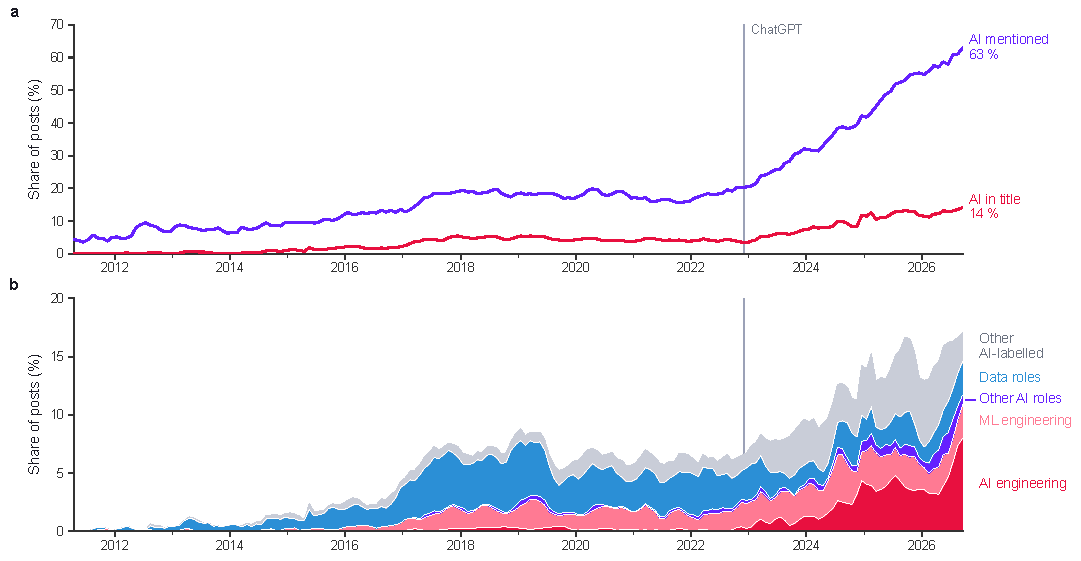
\includegraphics[width=\textwidth]{fig3_hn_series}
\caption{AI in international technology hiring, Hacker News ``Who is hiring'' 2011--2026, three-month centred means. (A) Share of posts mentioning AI anywhere and share whose role title is an AI or data title; vertical lines mark model releases. (B) Composition of AI and data titles by family.}\label{fig:hn}
\end{figure}

\Cref{fig:first} dates the first appearance of each canonical title and its fifth post. Data scientist and data engineer were established by 2013, machine-learning engineer by 2015, AI engineer by 2017. Forward deployed engineer reached five posts in \firstForwardDeployedEngineer{}, well before the generative wave, and grew \gForwardDeployedEngineer{} log points over the last twelve months with \hnLastForwardDeployedEngineer{} posts; generative AI engineer reached five posts in \firstGenaiEngineer{} and already declined (\gGenaiEngineer); AI agent engineer appeared in \firstAgentEngineer{}; AI governance in \firstAiGovernance{}; AI architect in \firstAiArchitect{}. The discovery of n-grams (\cref{fig:discovery}) confirms that the titles born after ChatGPT are mostly recombinations of ``AI'' with an existing role: \emph{applied AI engineer}, \emph{founding AI engineer}, \emph{AI product engineer}, \emph{full-stack AI engineer}. Among \nNgramsHN{} title n-grams with at least eight posts, \nNgramsNew{} first appeared after November 2022. In France, the most frequent AI title n-grams in 2026 are \emph{data scientist}, \emph{intelligence artificielle}, \emph{data IA}, \emph{AI engineer}, \emph{ingénieur IA}, \emph{développeur IA}, \emph{IA générative}, \emph{chef de projet IA} and \emph{IA agentique}.

\begin{figure}[t]
\centering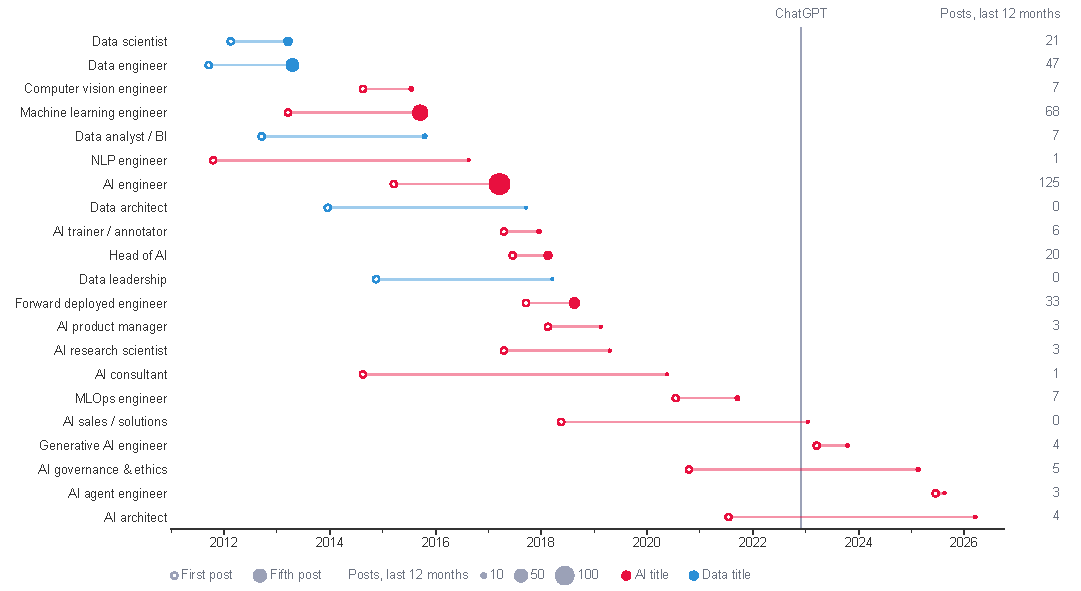
\includegraphics[width=\textwidth]{fig4_hn_first_appearance}
\caption{First appearance of each canonical AI and data title in international technology hiring. Open circle: first post; filled circle: fifth post, sized by the title's share of posts in the last twelve months; right column: posts in the last twelve months and log growth against the previous twelve.}\label{fig:first}
\end{figure}

\subsection{Emergence Index and lifecycle stages (\RQ{1}, \RQ{5})}\label{sec:index_res}
\Cref{fig:index} ranks the titles by the Emergence Index. AI engineer leads ($E=\EAiEngineer$) because it combines persistence, breadth (\frEmpAiEngineer{} French employers in 2026) and a title still growing in France; it is classified as established. Forward deployed engineer ($E=\EForwardDeployedEngineer$, \stageForwardDeployedEngineer) is the clearest case of a structurally new role: it was created by one company to put software in production at the client's site, spread to \hnLastForwardDeployedEngineer{} posts and 25 employers in the last twelve months internationally, and has reached \frForwardDeployedEngineer{} French postings from \frEmpForwardDeployedEngineer{} employers. Head of AI, AI architect, MLOps engineer and AI trainer are diffusing. Machine-learning engineer (\stageMlEngineer, growth \gMlEngineer) and data scientist (\stageDataScientist, \gDataScientist) are established and no longer growing internationally, consistent with relabelling toward ``AI engineer''. Generative AI / LLM engineer is \stageGenaiEngineer{} after a short life: \hnPrevGenaiEngineer{} posts in the previous twelve months, \hnLastGenaiEngineer{} in the last twelve, while \frGenaiEngineer{} French postings still use it. Prompt engineer has \frPromptEngineer{} French posting in 2026 and no international post in the last twelve months. Of \nStages{} titles, \nAppearing{} are appearing, \nDiffusing{} diffusing, \nEstablished{} established and \nFading{} fading.

\begin{figure}[t]
\centering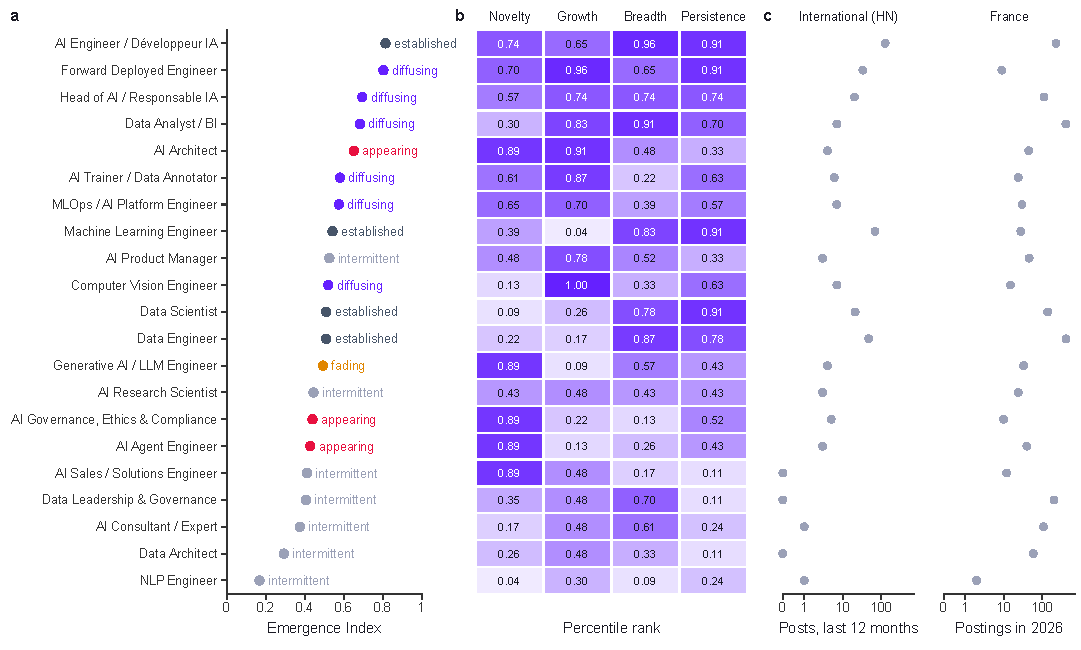
\includegraphics[width=\textwidth]{fig10_emergence_index}
\caption{Emergence Index of canonical AI and data titles. (A) Index and lifecycle stage. (B) Percentile ranks of the four components. Right: month of the fifth post, international posts in the last twelve months with log growth, French postings and employers in 2026.}\label{fig:index}
\end{figure}

\subsection{Diffusion in France: sectors, territories, contracts (\RQ{2})}\label{sec:fr}
AI is mentioned in \nAI{} of the \nFT{} French postings (\pAI\,\%), and \nCore{} carry an AI title (\pCore\,\%). \Cref{fig:breakdown} shows where the mentions concentrate. By sector, information and communication leads (\nafJ\,\%), followed by real estate (\nafL\,\%) and professional, scientific and technical activities (\nafM\,\%); construction is lowest (\nafF\,\%). By region, \^Ile-de-France (\idfShare\,\%) is more than twice the national share and concentrates \idfConc\,\% of AI postings for \idfJobs\,\% of all postings; the next region is \regSecond{} (\regSecondShare\,\%). At the department level, Hauts-de-Seine (\depHautsDeSeine\,\%) and Paris (\depParis\,\%) stand out (\cref{fig:map} in the appendix). By contract type, freelance and liberal missions mention AI in \conLIB\,\% of cases, against \conCDI\,\% of permanent contracts, \conCDD\,\% of fixed-term contracts and \conMIS\,\% of temporary-agency assignments. By establishment size, the share is flat below 500 employees and two to four times higher between 500 and 10\,000 employees. The top ten employers account for \topTenEmp\,\% of AI postings; the first is \topEmp{}, a freelance platform, with \topEmpN{} postings.

\begin{figure}[t]
\centering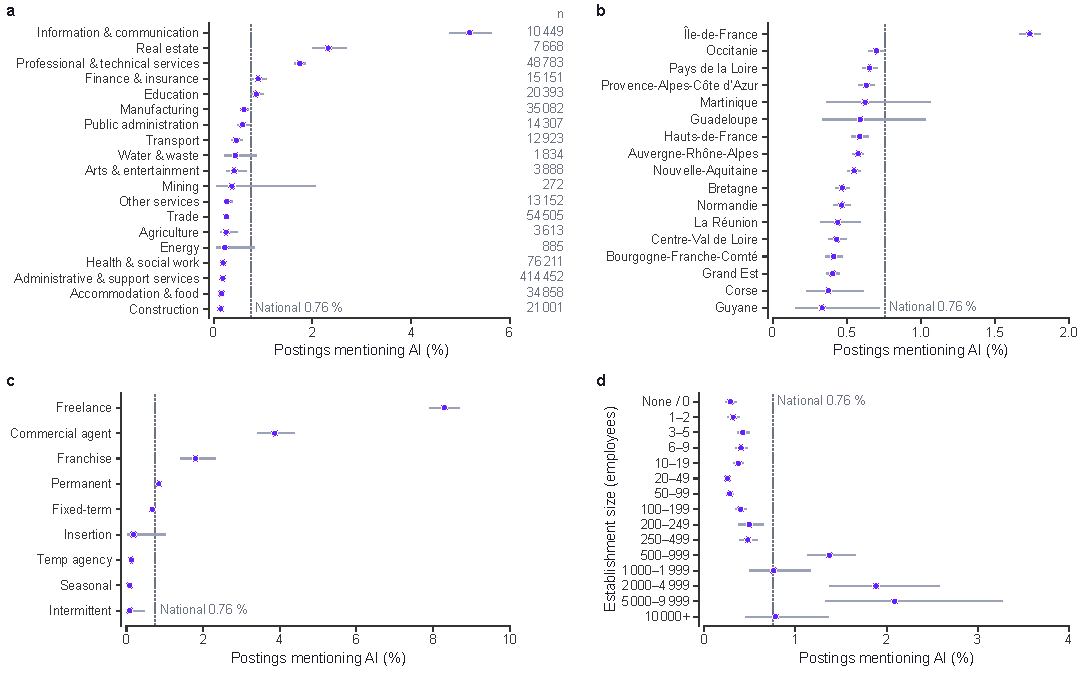
\includegraphics[width=\textwidth]{fig5_ft_ai_share_breakdowns}
\caption{Share of French postings mentioning AI, France Travail 2026, with Wilson 95\,\% intervals. (A) Employer sector. (B) Region of the workplace. (C) Contract type. (D) Establishment size.}\label{fig:breakdown}
\end{figure}

The second layer is large: \nAIoutside{} postings that mention AI, \pAIoutside\,\% of them, are not technology jobs. They are real-estate agents, accountants, teachers, sales representatives and administrative staff whose employers now expect the use of AI tools. The validation (\cref{sec:valres}) shows that in \aiJobShare\,\% of the confirmed mentions the reference concerns the job itself rather than the employer's presentation.

\subsection{Skill architecture (\RQ{3})}\label{sec:skills}
\Cref{fig:skills}A compares the skill families cited by AI-core postings, AI-related technology postings and other technology postings in France. AI-core postings cite AI/ML modelling skills in \skModelCore\,\% of cases and generative-AI skills in \skGenAICore\,\%, against \skModelTech\,\% and \skGenAITech\,\% for other technology jobs; cloud, DevOps and MLOps skills are cited in \skCloudCore\,\% of AI-core postings and software-engineering skills in \skSoftCore\,\%, so an AI job remains an engineering job. Governance, ethics and regulation skills appear in \skGovCore\,\% of AI-core postings. \Cref{fig:skills}B contrasts selected titles: the AI engineer profile is dominated by generative AI and software engineering, the data scientist by modelling and analysis, the data engineer by data engineering and cloud. \Cref{fig:skills}C shows the international shift inside AI posts: generative-AI skills rose from \hnGenAIpre\,\% of AI posts in 2022 to \hnGenAIlast\,\% in 2026, while classical modelling skills moved from \hnModelPre\,\% in 2019 to \hnModelLast\,\%. \Cref{fig:skills}D gives the co-occurrence network of the thirty most cited skills in French AI postings.

\begin{figure}[t]
\centering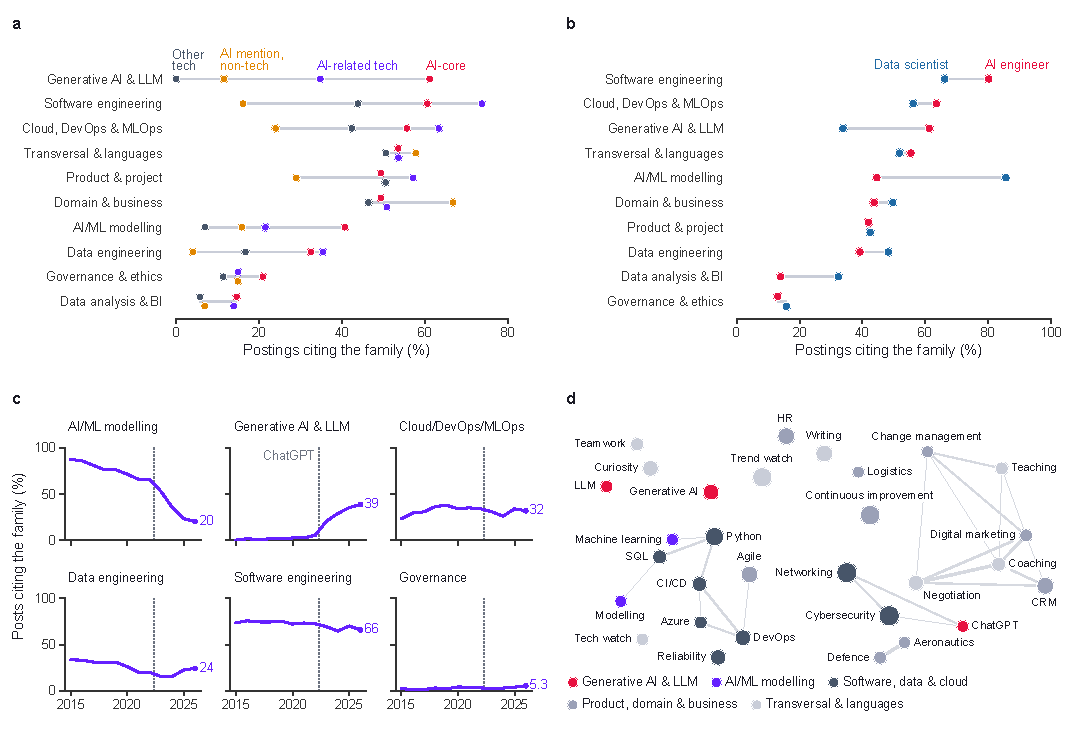
\includegraphics[width=\textwidth]{fig12_skills}
\caption{Skill families. (A) Share of postings citing at least one skill of each family, by segment, France 2026. (B) Profile of selected canonical titles. (C) Skill content of international AI posts by year. (D) Co-occurrence of the thirty most cited skills in French AI postings; node colour is the family, edges are Jaccard similarities above 0.18.}\label{fig:skills}
\end{figure}

\subsection{Salaries and experience (\RQ{4})}\label{sec:salary}
Among postings with a salary range, AI-related technology jobs advertise a median of \salAItech\,k\euro{} (n = \salNAItech), other technology jobs \salTech\,k\euro{} (n = \salNTech), a gross premium of \salPremAItech\,\%; AI-core jobs advertise \salCore\,k\euro{} (n = \salNCore) and the whole corpus \salAll\,k\euro{} (\cref{fig:salary}A). Experience is required in \expAItech\,\% of AI-related technology postings against \expTech\,\% of other technology postings; AI-core postings are more open to beginners (\expCore\,\% require experience), because the segment includes trainers, annotators and apprenticeships. A hedonic regression with region, contract, experience and establishment-size controls is \tg{planned} for the revised version.

\begin{figure}[t]
\centering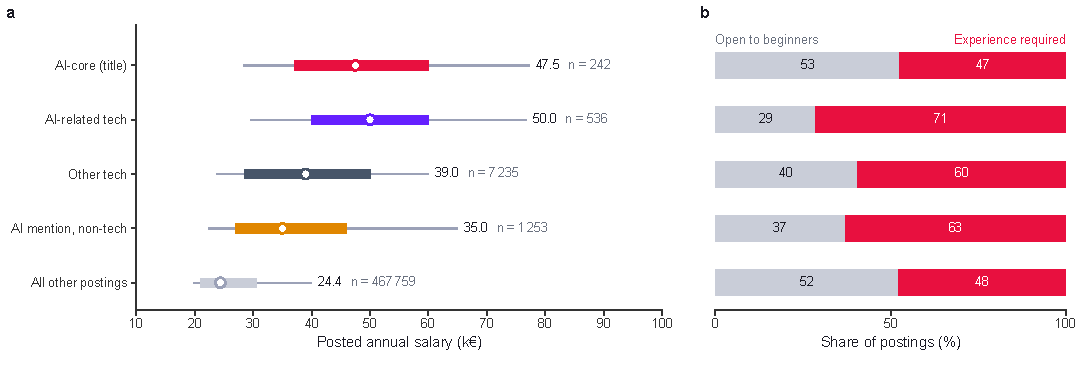
\includegraphics[width=\textwidth]{fig7_ft_salary_experience}
\caption{(A) Posted annual salaries by segment, France Travail 2026, midpoint of the posted range; boxes show quartiles, whiskers the 5th and 95th percentiles. (B) Experience requirement by segment.}\label{fig:salary}
\end{figure}

\subsection{The public sector (\RQ{5})}\label{sec:public}
In the \nCSP{} public-sector postings, AI mentions in titles and occupation labels rose from \cspFirst{} per 10\,000 postings in 2022 to \cspLast{} in 2026, a \cspRatio-fold increase, with a steeper slope after November 2022 (\cref{fig:csp} in the appendix). The most frequent canonical titles are data analyst, data scientist and data engineer; AI engineers and researchers appear mostly in research organisations and universities.

\subsection{Validation}\label{sec:valres}
On the 1\,000 annotated postings, the technology-scope rule reaches a precision of \precIsTech\,\% and a recall of \recIsTech\,\% ($\kappa=\kappaIsTech$). The AI-mention rule reaches a precision of \precAiAny\,\% and a recall of \recAiAny\,\% ($\kappa=\kappaAiAny$); the AI-title rule a precision of \precAiCore\,\% and a recall of \recAiCore\,\% ($\kappa=\kappaAiCore$). When the judge and the rule both assign a canonical title, they agree in \canonAgree\,\% of the \nCanonBoth{} cases; disagreements are mostly between neighbouring titles (AI engineer against machine-learning engineer, data analyst against data scientist). The residual false positives of the AI-mention rule are brand names containing ``AI'', the word \emph{copilote} used as a metaphor, and AI mentioned only in the employer's presentation.

\section{Discussion}\label{sec:discussion}
\paragraph{Relabelling and new work} The evidence supports a two-speed reading of the AI wave. Most of the titles that appeared after 2022 recombine ``AI'' with an existing role, and the decline of machine-learning engineer and data scientist internationally while AI engineer keeps growing is what relabelling looks like in postings. A minority of titles are new work in the sense of \citet{autor2024}: forward deployed engineer bundles software engineering with on-site deployment and client-facing work, AI agent engineer bundles orchestration and evaluation of autonomous systems, and AI governance bundles law, risk and model auditing. These titles have distinct skill profiles and diffuse across employers, which the Emergence Index captures through breadth rather than volume.

\paragraph{Diffusion outside technology jobs} The largest effect in France is not in technology occupations. More than half of the postings that mention AI are ordinary jobs, and the share is highest in freelance missions, where demand adjusts fastest. For training providers, this suggests that AI literacy for non-technical occupations is a larger market than AI specialist training. For statistical agencies, it suggests measuring AI diffusion at the level of the posting and not only of the occupation.

\paragraph{Limits} The French series is a 2026 cross-section; the daily harvest and the JOCAS data will turn it into a series. France Travail under-represents executive jobs, so French counts of AI-titled jobs are lower bounds; Adzuna's live counts (16\,049 IT ads against 8\,423 France Travail IT offers on the same day) indicate that the specialised boards carry roughly twice the volume. The rules are lexical; the embedding extractor and the renaming test are the next step. The judge is a language model, with a human review of 200 items; its errors are documented and do not favour the rules.

\section{Conclusion}\label{sec:concl}
We built an open corpus of \nAll{} million postings, measured the emergence of AI occupations with an index that rewards diffusion rather than volume, and validated the measurement. AI is now mentioned in \hnAIlast\,\% of international technology hiring posts and in \pAI\,\% of all French postings; the AI-titled layer is thin and mostly relabelled, with a few structurally new roles; the AI-mention layer is thick and largest outside technology jobs. The pipeline runs monthly and feeds a public observatory; the next versions will add the French time series, the embedding-based skill extractor, the renaming test and the hedonic salary model.

\section*{Data and code availability}
The lexicon, the scope rules, the aggregated result tables and the code are released at the observatory website; the France Travail and public-sector postings are available from their open APIs and portals; Hacker News posts are public.

\section*{Acknowledgements}
\noindent [Funding and data providers to be completed.]

\bibliographystyle{elsarticle-harv}
\bibliography{refs}

\appendix
\section{Additional figures}\label{app:figs}
\begin{figure}[h]
\centering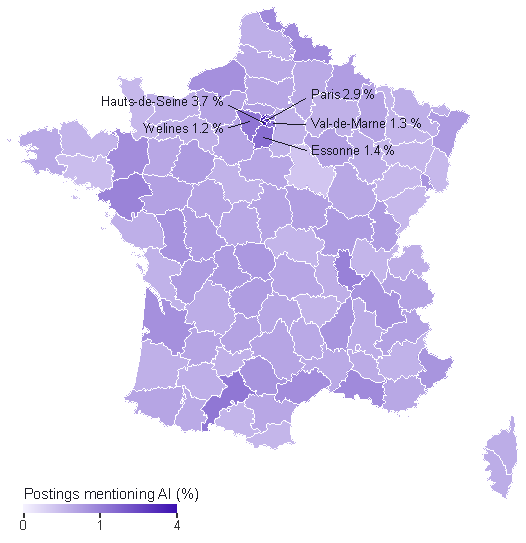
\includegraphics[width=0.62\textwidth]{fig6_ft_map_dept}
\caption{Share of postings mentioning AI by département, France Travail 2026.}\label{fig:map}
\end{figure}
\begin{figure}[h]
\centering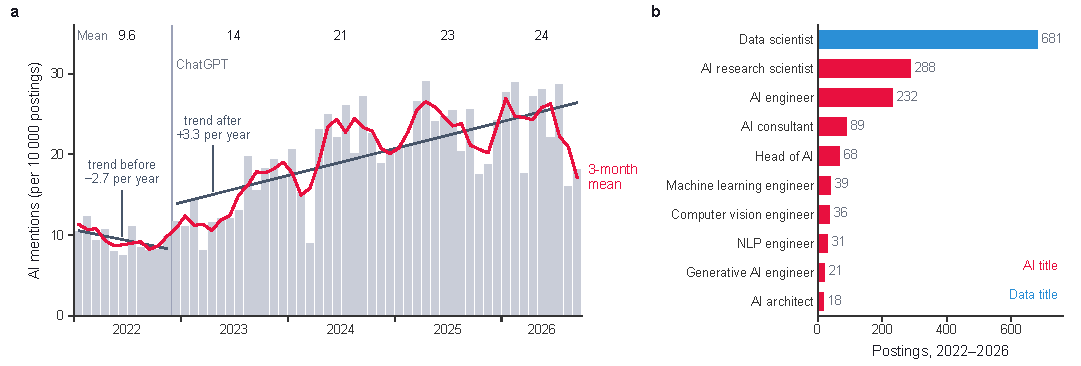
\includegraphics[width=\textwidth]{fig9_csp_public_sector}
\caption{AI in French public-sector postings, Choisir le Service Public, 2022--2026. (A) AI mentions per 10\,000 postings, monthly, with pre- and post-ChatGPT linear trends. (B) Canonical titles.}\label{fig:csp}
\end{figure}
\begin{figure}[h]
\centering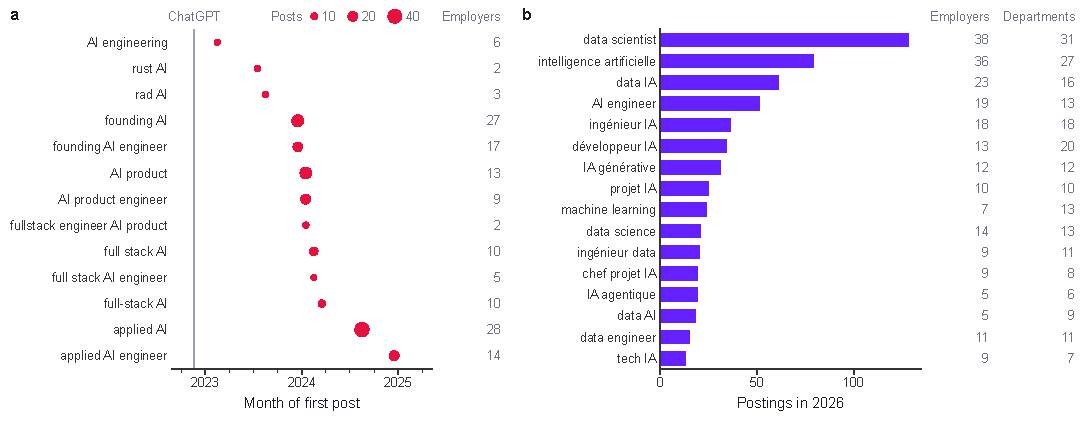
\includegraphics[width=\textwidth]{fig11_discovered_titles}
\caption{Data-driven discovery of AI title n-grams. (A) N-grams whose first post is after November 2022 (Hacker News). (B) Most frequent AI title n-grams in French AI-core postings, 2026.}\label{fig:discovery}
\end{figure}
\begin{figure}[h]
\centering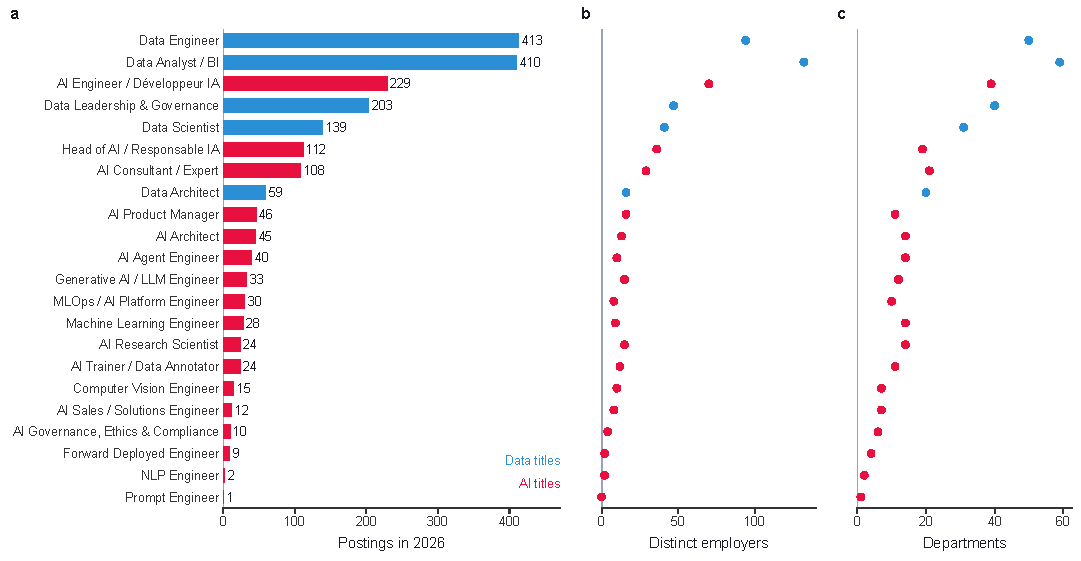
\includegraphics[width=\textwidth]{fig8_ft_canonical_titles}
\caption{Canonical AI and data titles in French postings, 2026: postings, employers, departments, share in \^Ile-de-France and posted median salary.}\label{fig:canon}
\end{figure}
\end{document}
